\documentclass{article}
\usepackage[czech]{babel}
\usepackage{fancyhdr}
% \usepackage[]{showframe}
\usepackage[a4paper,top=2cm,bottom=2cm,left=3cm,right=3cm,marginparwidth=1.75cm]{geometry}
\usepackage{graphicx}
\usepackage{rotating}
\usepackage{hyperref}


\begin{document}
\graphicspath{{ fig/ }}
\thispagestyle{fancy}

% Title page
\newgeometry{bottom=5cm}
\begin{center}
    \textsc{ \huge{Vysoké učení technické v Brně} } \\ [0.5cm]
    \textsc{ \huge{Fakulta informačních technologií} } \\ [5cm]
    \textsc{ \huge{Úvod do softwarového inženýrství} } \\ [0.5cm]
    \textsc{ \huge{2022/2023} } \\ [3cm]
    \huge{Projekt č. 1 -- Model informačního systému} \\ [2cm]
    \textbf{ \huge{Zadání č. 59 -- Sociální síť} }
\end{center}


% Remove header line
\fancyhf{} %
\renewcommand{\headrulewidth}{0pt}

% Footer
\fancyfoot[L]{\Large{ Jakub Bláha (xblaha36), \\ Veronika Čalkovská (xcalko00), \\ Jan Klanica (xklani00), \\ Tomáš Kocí (xkocit00), \\ Pavel Lukl (xluklp00) }}
\fancyfoot[R]{\Large{Brno, \today} }

\restoregeometry
\newpage

\tableofcontents
\listoffigures

\newpage

% Assignment
\section{Zadání -- Sociální síť}

Představte si, že jste Mark Zuckergerg v roce 2004 a chystáte se vytvořit sociální síť, která bude známá po celém světě. Jelikož chcete o svým uživatelích vědět maximum informací, budete o nich chtít uložit veškeré jejich základní informace včetně škol, které navštěvovali, bydliště, zaměstnání, kontaktu, rodiny a vztahů, atd. Jedná se o sociální síť, a tak svých uživatelům dovolíte, aby vzájemně vytvářeli (leckdy) imaginární přátelství mezi sebou. Abyste o svých uživatelích věděli všechno nejen vy, ale i ostatní uživatelé, vytvoříte zeď, na kterou budou jednotliví uživatelé publikovat příspěvky, které budou mít obsah, datum, místo a čas publikování a můžou v nich být označeni i jiní uživatelé. Aby si uživatelé mohli sdílet nejen své duchapřítomné příspěvky, ale také fotky svých domácích mazlíčků a naleštěných dvoukolových miláčků, dovolíte jim vytvářet i alba fotek, které budou mít svůj název, nastavení soukromí a popis. Na jednotlivých fotkách mohou být označení různí uživatelé a bude u nich uveden čas, datum a místo pořízení a jedna z fotek bude vždy titulní fotka alba. Navíc může být fotka pořízena v rámci nějaké akce. Uživatelé si mohou prostřednictvím konverzací s jistým názvem, do níž můžou být zapojeni dva a více uživatelů, vyměňovat zprávy, které budou mít svůj obsah, datum, čas a místo zaslání. Aby vaší uživatelé neseděli přeci jen stále za obrazovkami svých notebooků, dovolíte jim vytvářet akce, které se konají na určitém místě, v určitý čas a den. Účastníci akce by měli znát, o jakou akci se jedná a pokud se jim akce zalíbí, tak se mohou akce, ať už jen virtuálně, či skutečně zúčastnit.

\newgeometry{bottom=0cm,top=0cm,left=0cm,right=0cm}

% Use case
\begin{figure}[p]
    \centering
    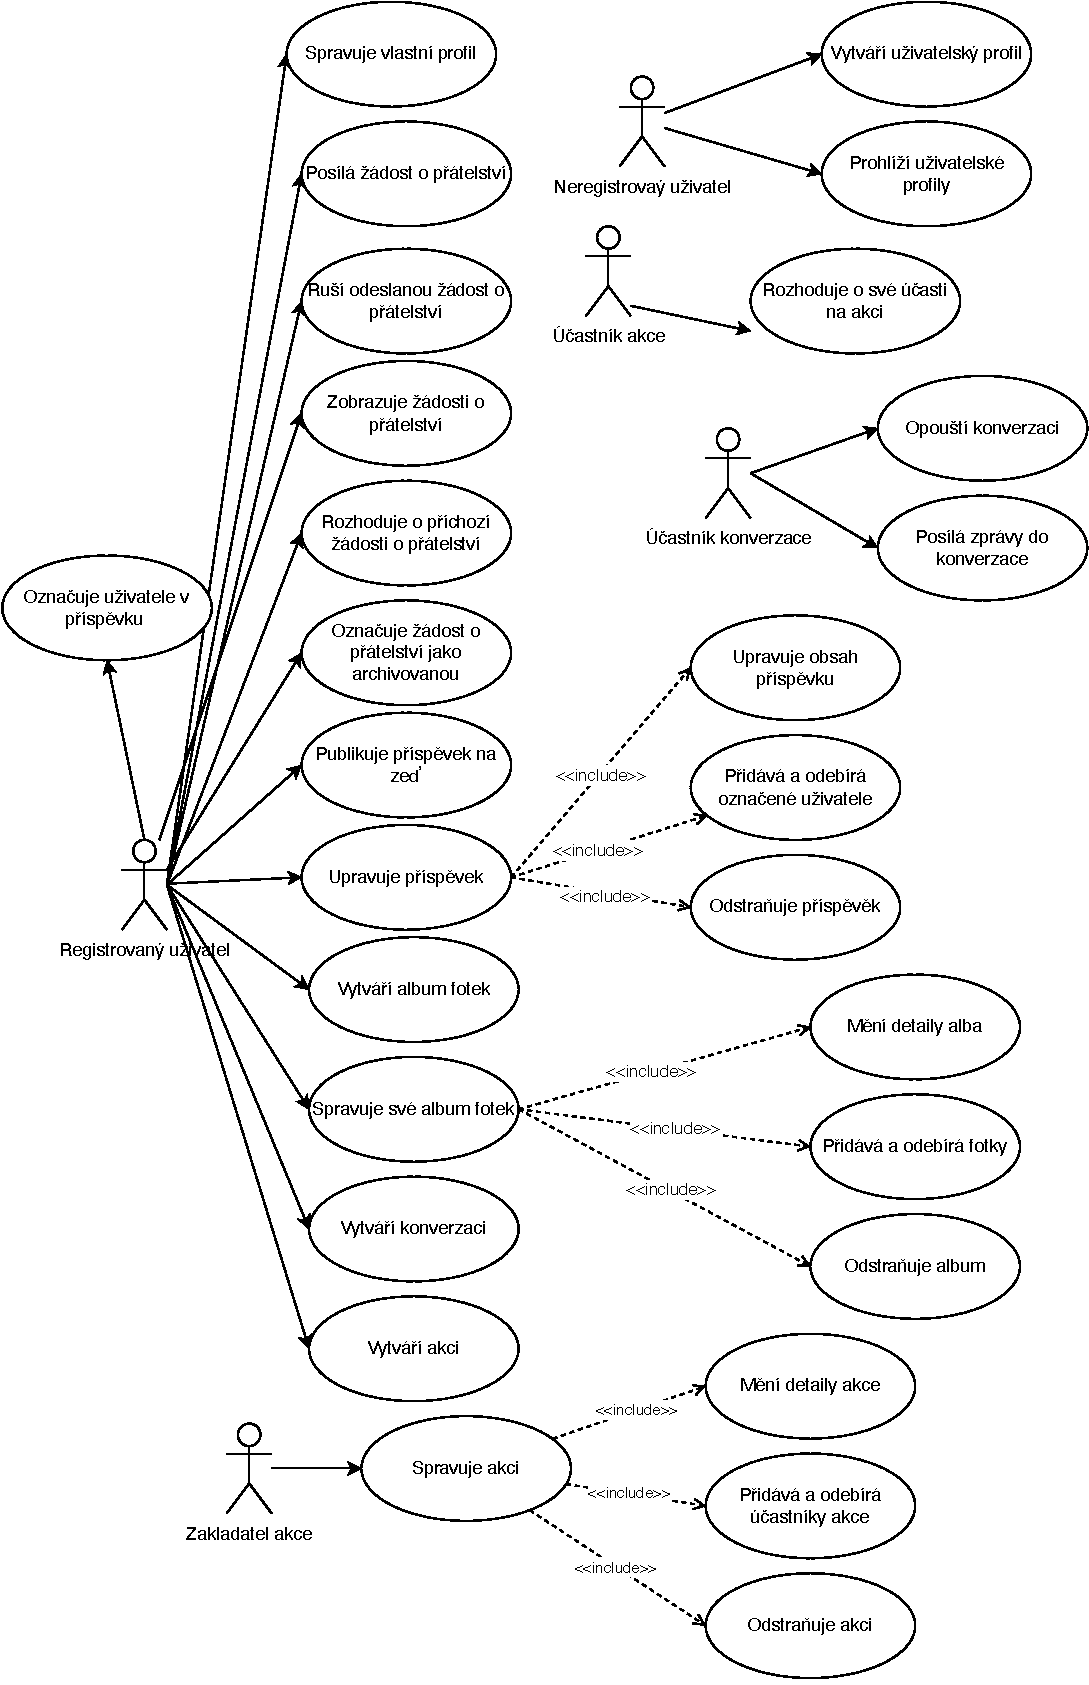
\includegraphics[scale=0.9]{fig/use-case.drawio.pdf}
    \caption{Use case diagram}
\end{figure}

% ER
\begin{figure}[p]
    \centering
    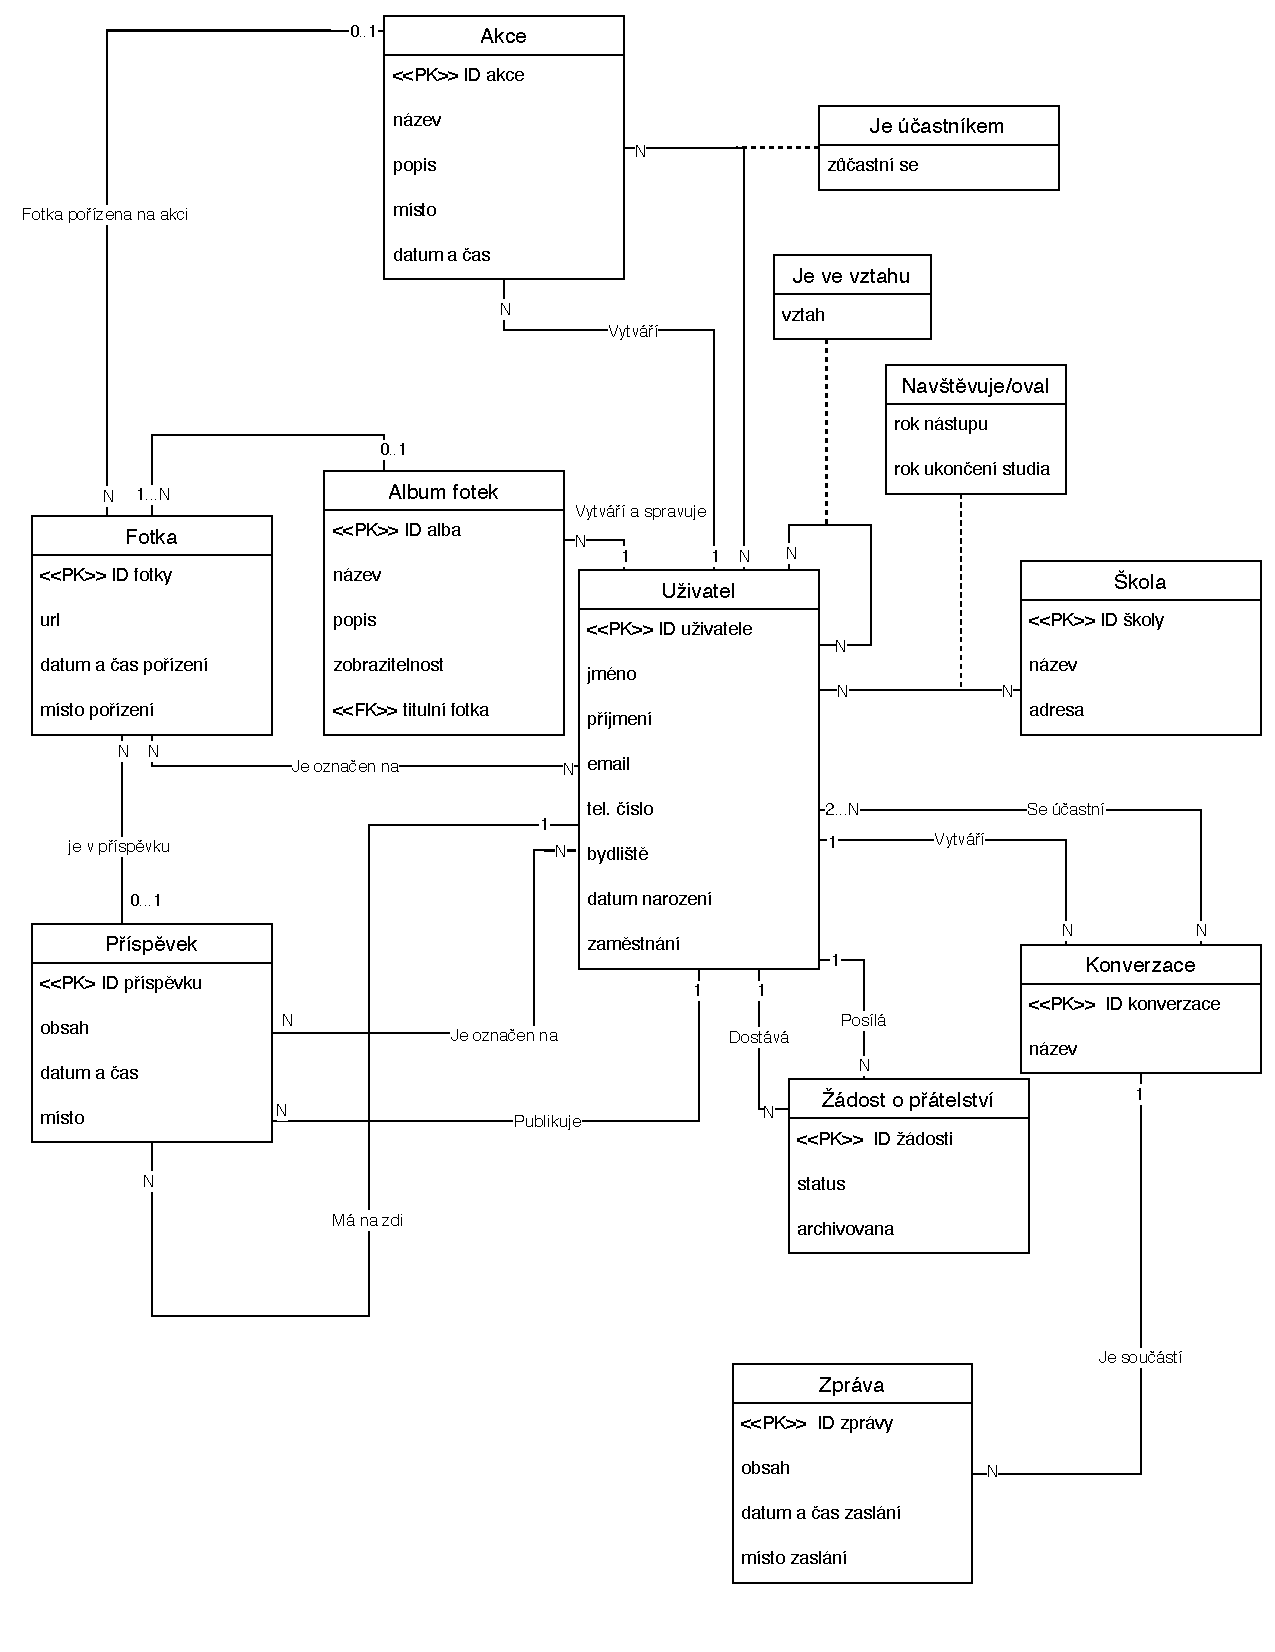
\includegraphics[scale=0.9]{fig/er.drawio.pdf}
    \caption{Entity relationship diagram}
\end{figure}

% Tridy
\begin{sidewaysfigure}[p]
    \centering
    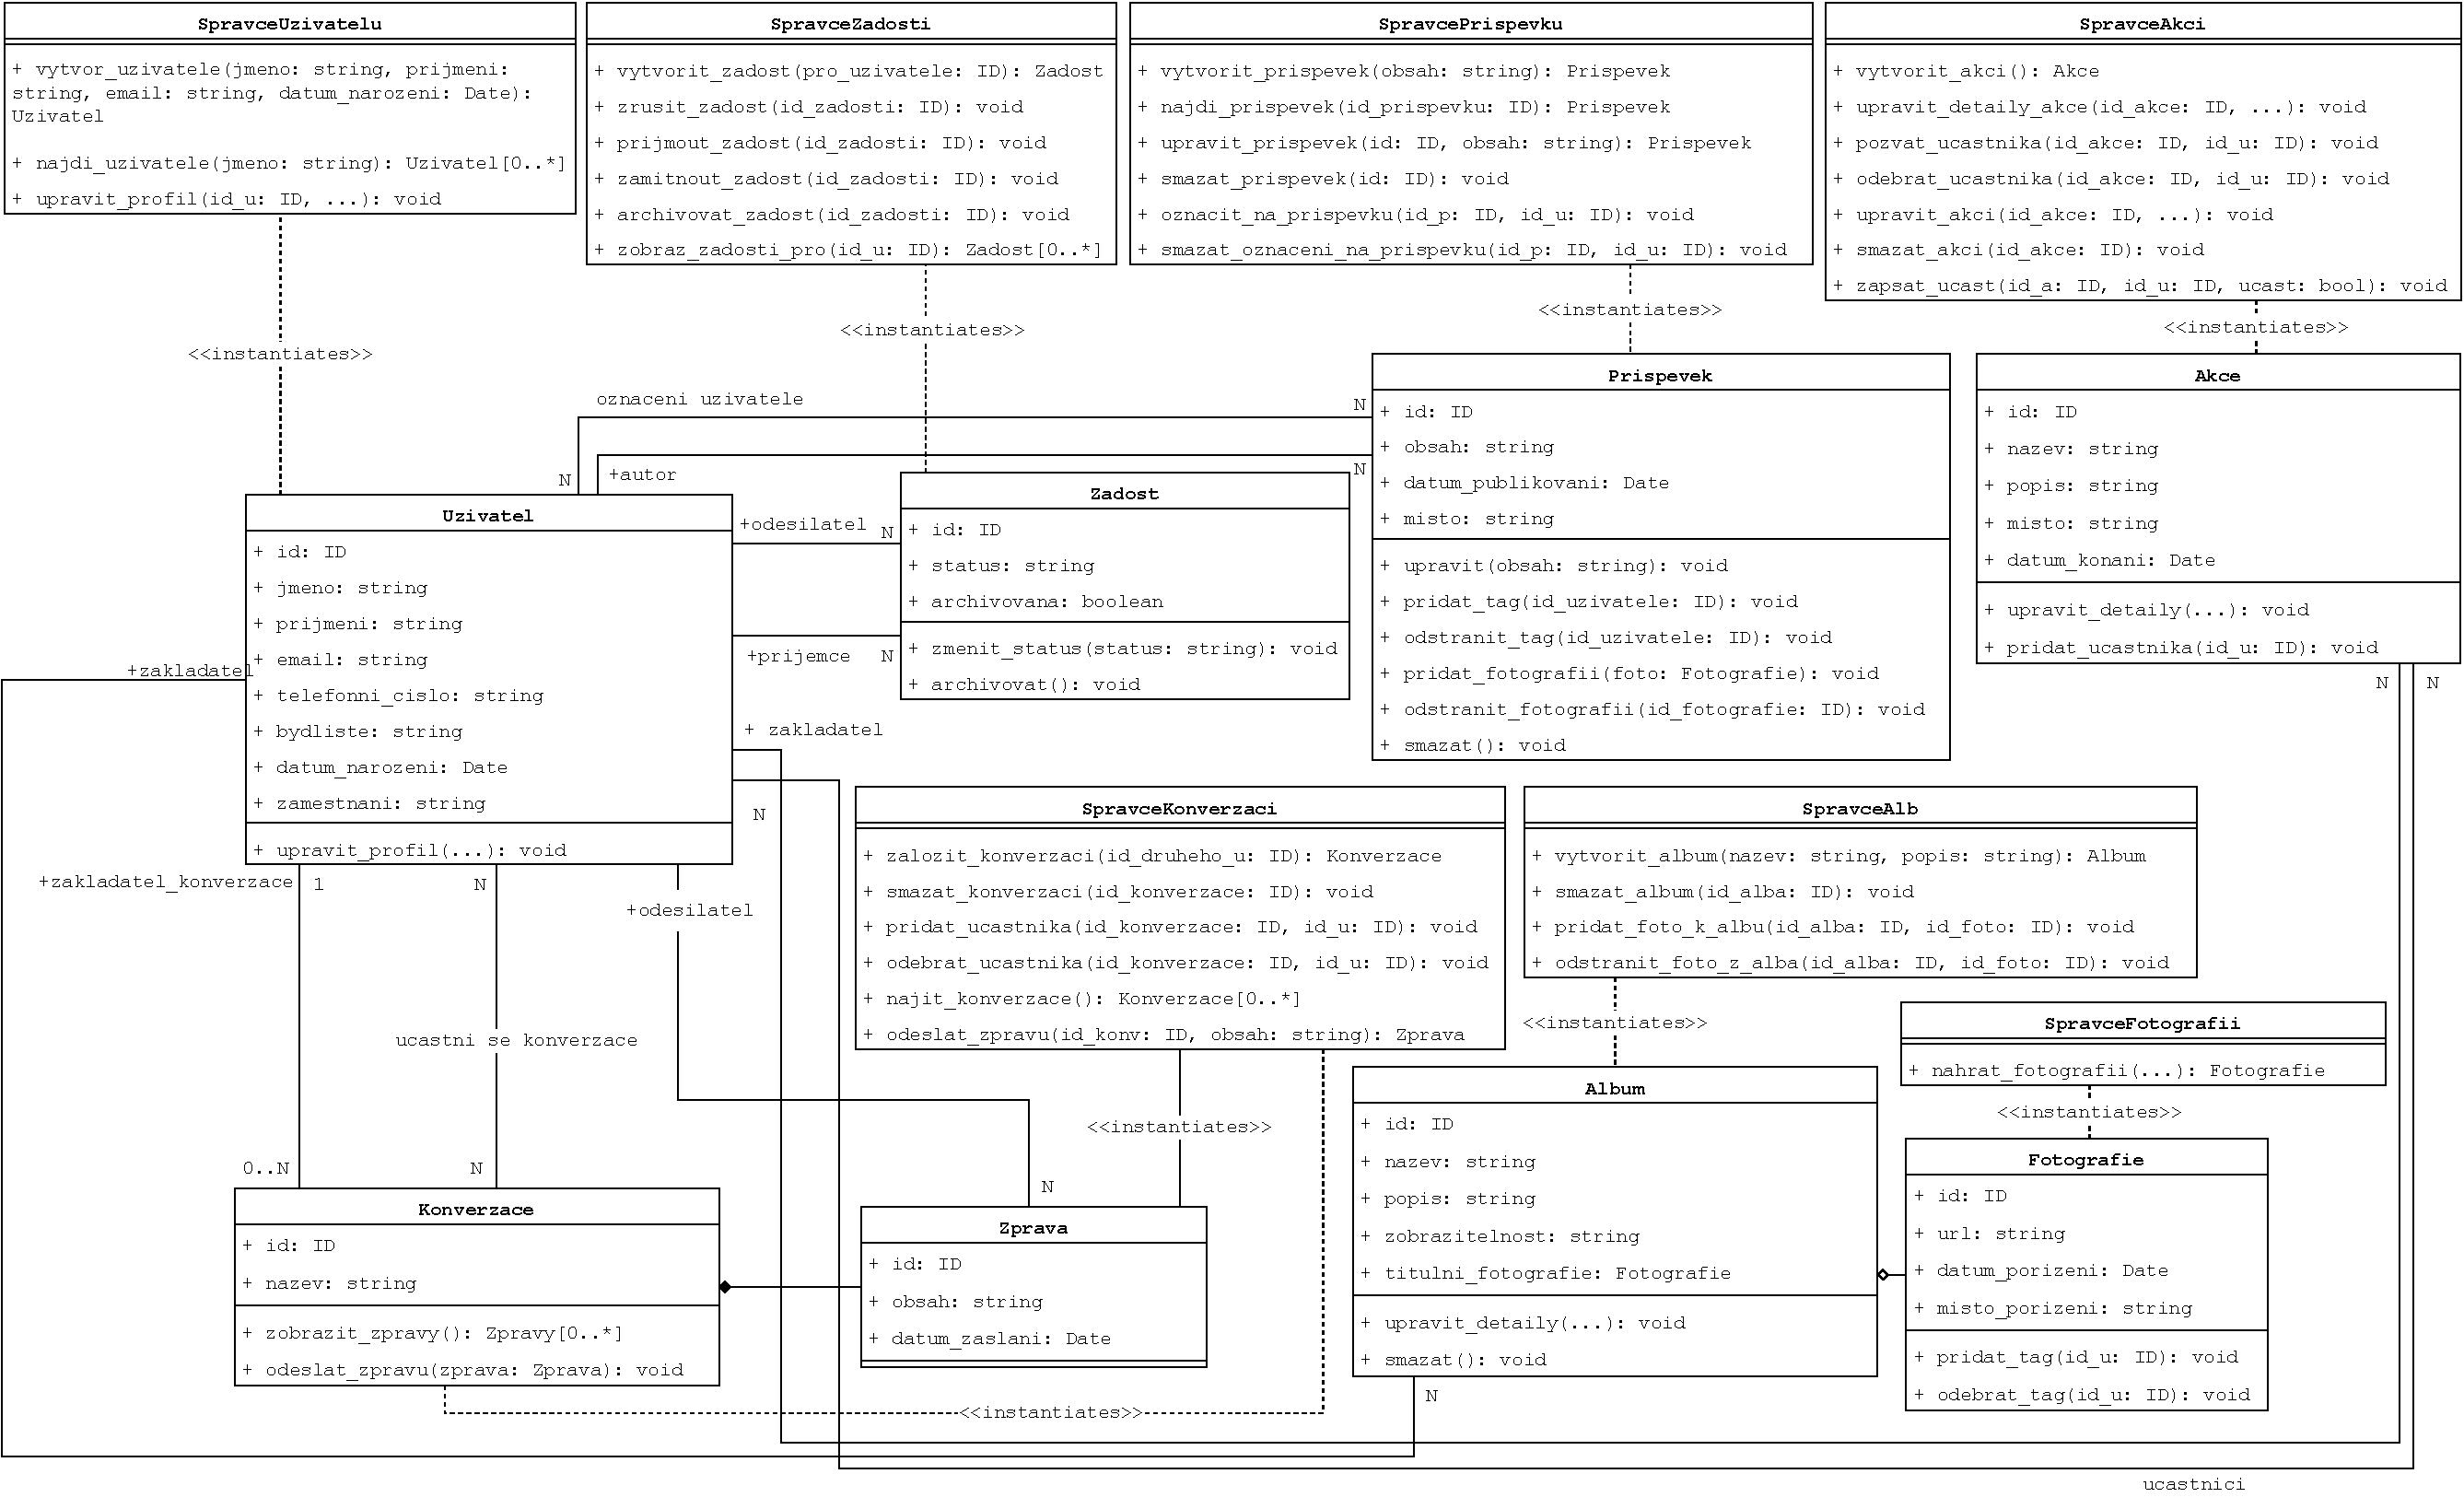
\includegraphics[scale=0.65]{fig/tridy.drawio.pdf}
    \caption{Diagram Tříd}
\end{sidewaysfigure}

% Sekvencni
\begin{figure}[p]
    \centering
    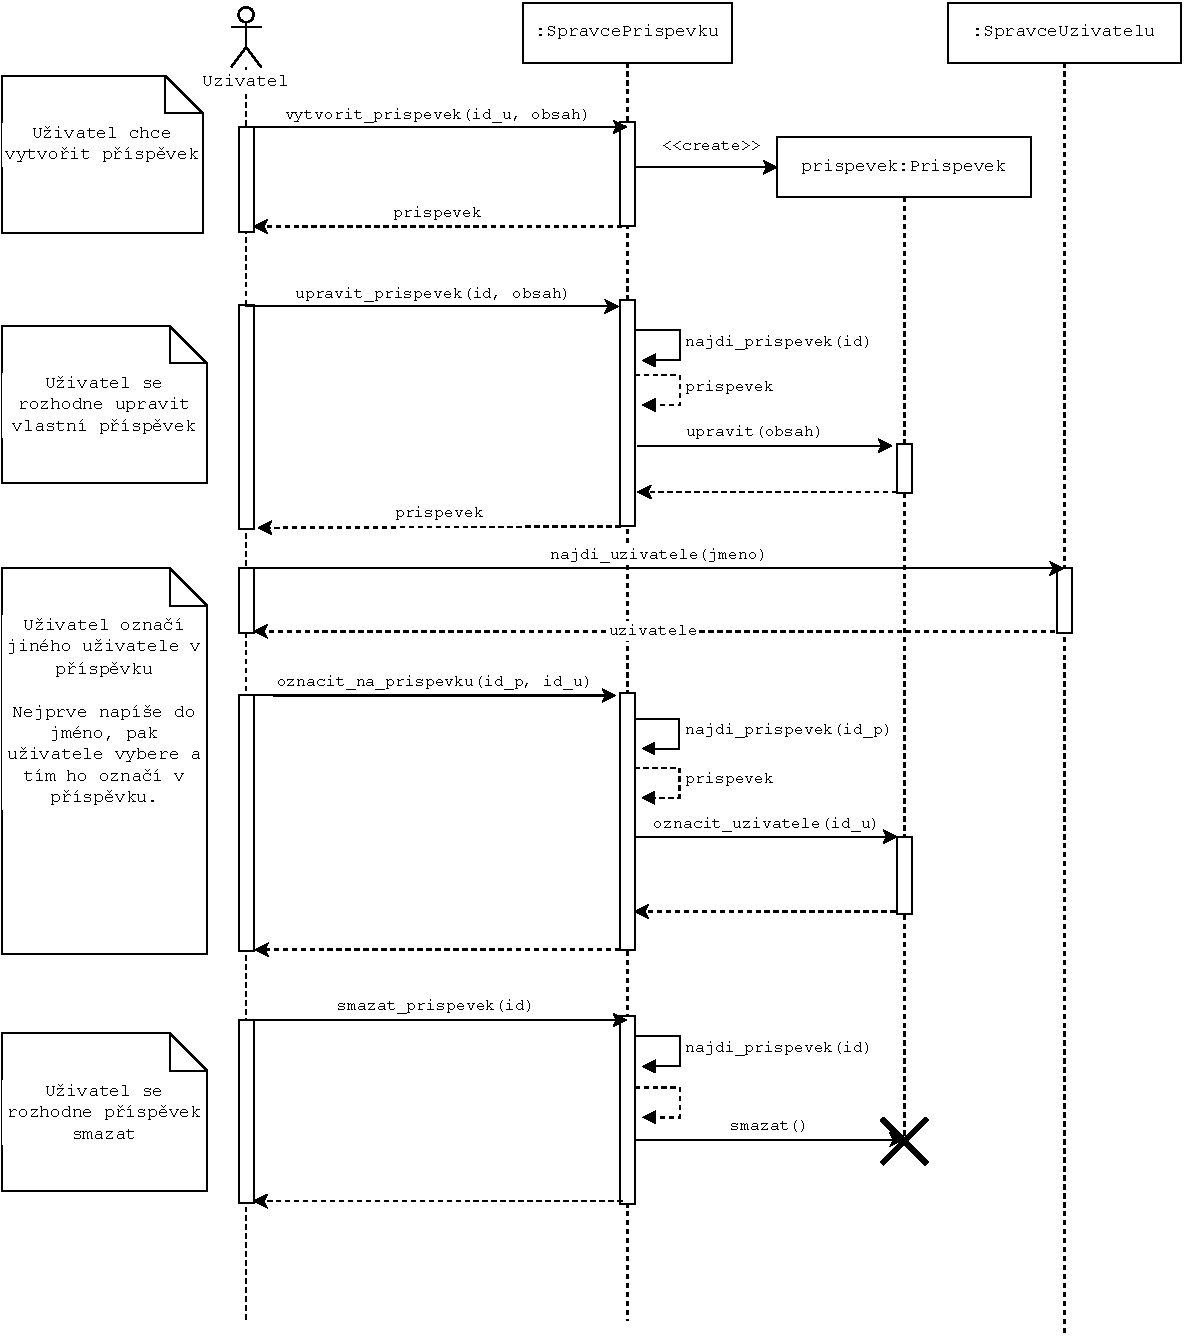
\includegraphics[scale=0.9]{fig/sekvencni.drawio.pdf}
    \caption{Sekvenční diagram}
\end{figure}

% Komunikace
\begin{figure}[p]
    \centering
    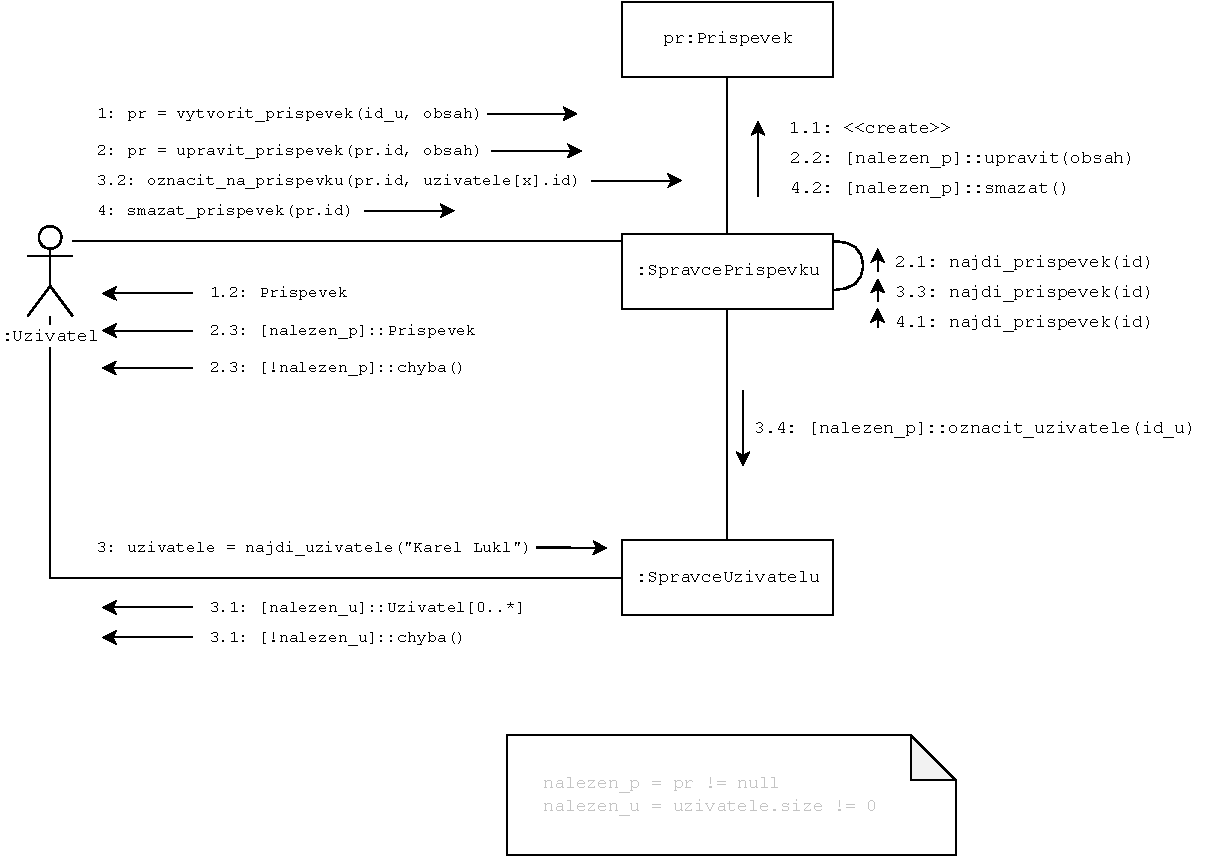
\includegraphics[scale=0.9]{fig/komunikace.drawio.pdf}
    \caption{Diagram komunikace}
\end{figure}

\clearpage

% Stavovy
\begin{figure}[p]
    \centering
    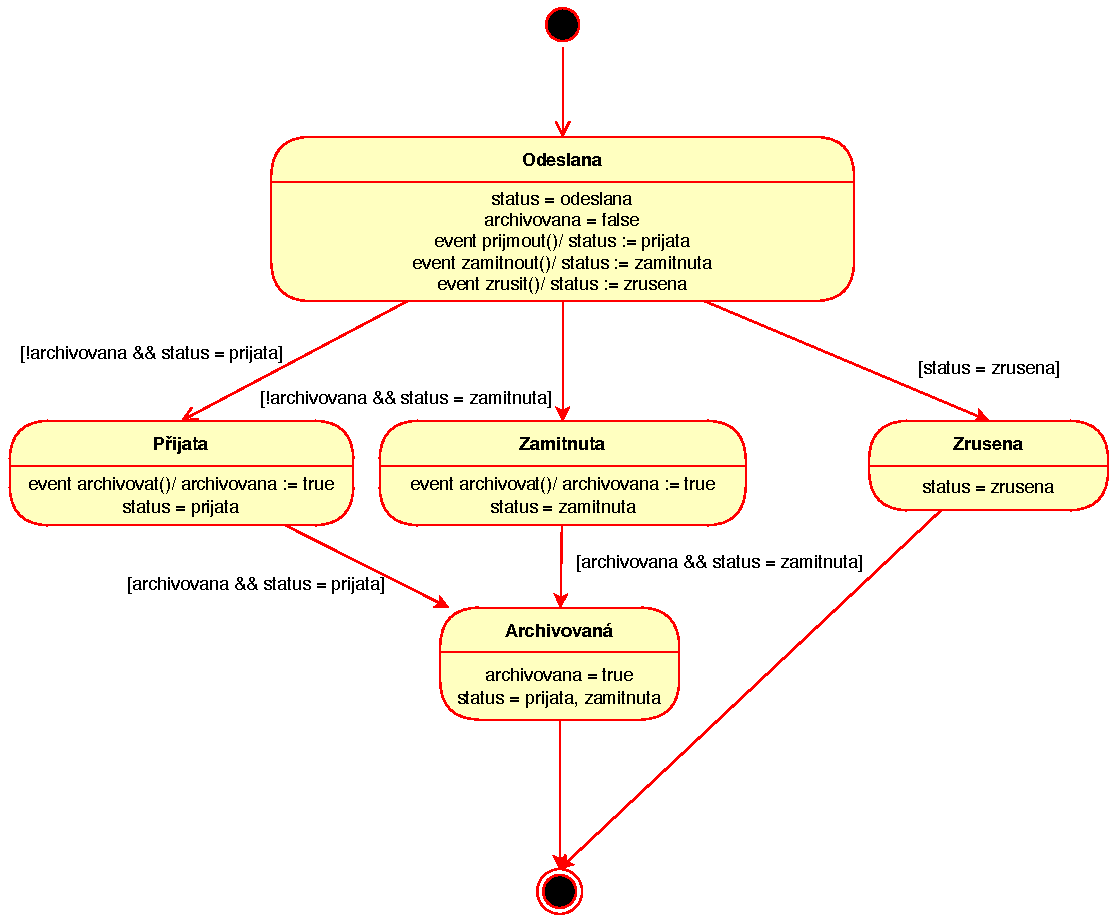
\includegraphics[scale=0.9]{fig/stavy.drawio.pdf}
    \caption{Stavový diagram}
\end{figure}

\restoregeometry
\end{document}